\documentclass{evolang11}
\usepackage{graphicx}
\usepackage{url}

\begin{document}

\title{PRODUCING A PAPER USING LATEX}

\author{ANONYMOUS AUTHOR 1}

\address{University Department, University Name \\ City, Country\\email@university}

%\author{ANONYMOUS AUTHOR 2, ANONYMOUS AUTHOR 3}

%\address{University Department, University Name \\ City, Country\\email2@university, email3@university}  

\maketitle

\abstracts{This is where the abstract should be placed. It should consist of one paragraph giving a concise summary of the material in the article below. Note that this year, the review process will be double-blind, so initial submissions should be anonymous and no author details should be added above. However, to avoid problems with page limits, please do include the appropriate number of placeholders for authors. If multiple authors share an address, their names can be on the same line with a common address. Please avoid footnotes in the abstract or title -- acknowledgements for funding bodies etc. are to be placed in a separate section at the end of the text. An abstract is \textbf{not} required for short paper submissions (max. length 2 pages).}

\section{Guidelines}

\subsection{General Guidelines}

We have provided eight files for use when producing a paper using latex. You can download these files at: 

\begin{quote}
\url{http://www.evolang.org/stylesheets/}
\end{quote}

\begin{enumerate}

\item {\em evolang11.tex} --- the source for this document. 

\item {\em evolang11.pdf} --- PDF generated from {\em evolang11.tex}.

\item {\em evolang11.png} --- the figure file.

\item {\em evolang11.bib} --- the bibliography file.

\item {\em evolang11.cls} --- the class file that provides the higher
level latex commands for the proceedings. \textbf{Don't change the contents of this file.}
 
\item {\em apacite.bst} --- the APA bibliography style file.
  
\item {\em apacite.sty} --- the package handling citations.

\item {\em apacite.pdf} --- documentation for the APA packages.

\end{enumerate}

You can delete our sample text and replace it with your own
contribution to the volume, although we recommend that you keep an
initial version of the file for reference.  These files should work with
standard latex2e.

\subsection{Double-Blind Peer Review}

This year, the review process will be double-blind.  Authors will not be told who reviews their paper and reviewers will not be told who the authors of the papers are.  Please keep in mind these guidelines for keeping your paper anonymous:

\begin{enumerate}
\item  \textbf{Do not include the names and affiliations of authors in the paper}

Authors will add names and affiliations after the paper has been reviewed and accepted.  However, keep in mind that names and affiliations will take up space.  We suggest that authors include anonymous placeholders for names and affiliations to avoid problems with page limits (e.g. ``AUTHOR BBBBB \& AUTHOR CCCCC'').

\item \textbf{Try not to reveal the identity of the authors indirectly}

This can include the following steps:

\begin{itemize}
\item Use third person to refer to previous work by the authors.  e.g. instead of ``As we have previously shown, language is a complex system (Jones, 2012)'' use ``As was previously shown, language is a complex system (Jones, 2012)'', or more simply ``Language is a complex system (Jones, 2012)''.
\item Do not eliminate essential self-references or other references but limit self-references only to papers that are relevant for those reviewing the submitted paper.
\item Make sure figures do not contain any affiliation related identifier.
\end{itemize}

\end{enumerate}

If the paper is accepted the authors will be required to submit a camera-ready version.  In the camera-ready version, the steps above can be reversed and author names, affiliations and acknowledgements etc. may be added.  \textbf{Again, please make sure that the papers will adhere to the space limitations once these changes are made.}  Of course, given the small size of the field it may not be possible to completely prevent reviewers from guessing the identity of the authors.  


\subsection{Headings and Text}

Please preserve the style of the headings, text font and line spacing
in order to provide a uniform style for the proceedings volume.  Note
that page numbers should not be included --- the final pagination of
the volume will be done by the editors.


\subsection{References and Citations}

References and citations should be in the APA style, using the {\em
  apacite.sty} and {\em apacite.bst} files provided.  We have included
examples of reference style for various publication types in the
References section and in {\em evolang11.bib}.

\begin{description}
\item [Citation Example 1:] \citeA{pinker_90_natural} argue that \ldots
\item [Citation Example 2:] It has been argued \cite{pinker_90_natural} that \ldots
\end{description}
\nocite{tomasello_03_constructing,hauser_03_uniquely}

For details on more complex citation commands, please consult {\em apacite.pdf}.

\subsection{Footnotes}

Footnotes are denoted by a character superscript in the
text.\footnote{This is a footnote.}

\subsection{Equations}

Equations should be centered and numbered consecutively, as in
Eq.~(\ref{eq:simple_equation}).

\begin{equation}
p = q + r
\label{eq:simple_equation}
\end{equation}

\subsection{Tables}

Tables should have a uniform style throughout the paper.  We would
prefer the border lines to be of the style shown in Table~\ref{table1}
--- single lines at top and bottom, no vertical lines at left or
right.  Placement of inner lines is left to your judgement, but it
generally looks better if they are kept to a minimum.

Table captions should be placed at the top of the table, and are
generated using the $\backslash$tablecaption command.  The text within
the table should be $\backslash$footnotesize.


\begin{table}[ht]
  \tablecaption{An example table.  This caption is generated using the
    $\backslash$tablecaption environment, and the table itself is in
    $\backslash$footnotesize.}
{\footnotesize
\begin{tabular}{@{}cccc@{}}
\hline
 & Column 1 & Column 2 & Column 3\\
\hline
Row 1 & entry & entry & entry \\
Row 2 & entry & entry & entry \\
Row 3 & entry & entry & entry \\

\hline
\end{tabular}\label{table1}}
\end{table}


\subsection{Figures/Illustrations/Images}

It is best to embed the figures in the text where they are first cited,
e.g. see Fig.~\ref{inter}. Please ensure that all labels in the
figures are legible regardless of whether they are drawn electronically or manually.  Very large figures and tables should be placed
on a page by themselves.


\begin{figure}[ht]
\begin{center}
\scalebox{0.6}{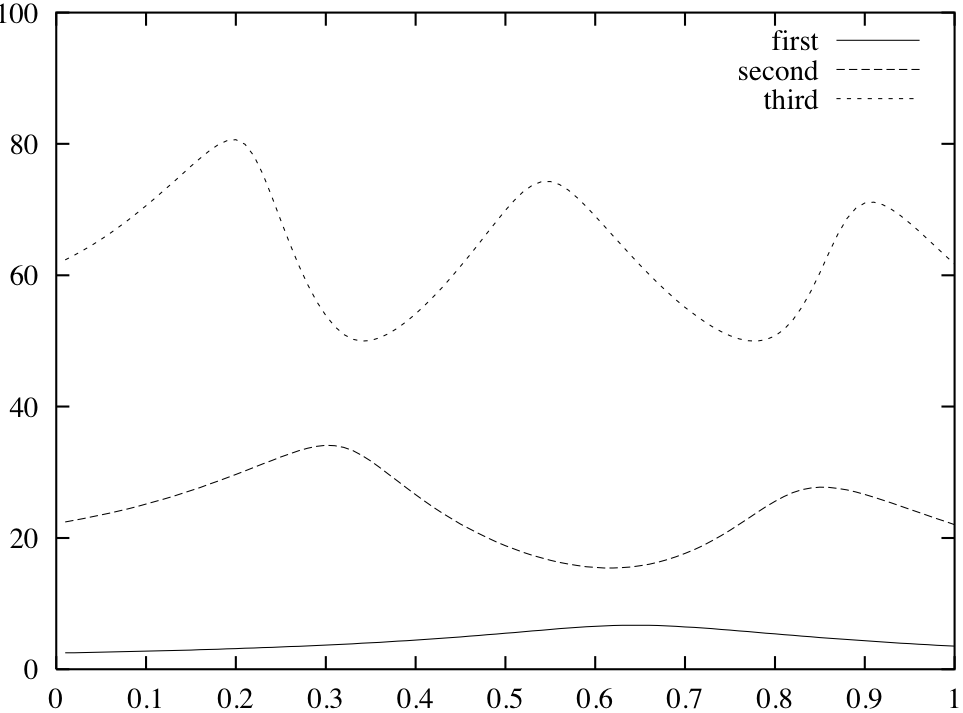
\includegraphics{evolang11.png}}
\end{center}
\caption{{\footnotesize An example graph.  All labels are legible, and
    this caption is in $\backslash$footnotesize. \label{inter}}}
\end{figure}

The caption heading for a figure should be placed below that figure.
The caption text should be $\backslash$footnotesize.

\section{Supplementary Materials}

There will be some support for supplementary materials.  All information necessary to understand and evaluate the submission should be included in the main paper.  Reviewers will not see the supplementary materials.  However, authors are encouraged to make data or code available for the final publication.  All supplementary materials should be submitted within a single zip file, which should also include a readme file describing the contents.  Supplementary materials should be referenced in the main text (e.g. ``see supplementary materials'').


\section*{Acknowledgements}

If you wish to acknowledge funding bodies etc., the acknowledgements
may be placed in a separate, unnumbered section at the end of the
text, before the Appendices.

\appendix

\section{Appendices}

Try to avoid using appendices.  If more than one Appendix is necessary
then set headings as Appendix~A, Appendix~B, etc.  Appendices should
come before the references. Number equations occurring in the Appendix according to appendix number, e.g. (A.1), (A.2), etc.

\bibliographystyle{apacite}
\bibliography{evolang11} 

\end{document}
